\documentclass[a4paper,12pt]{article}
\usepackage[margin=0.6in]{geometry}
\usepackage[latin1]{inputenc}
\usepackage[english]{babel}
\usepackage{amsmath}
\usepackage[makeroom]{cancel}
\usepackage{amsmath,tabu}
\usepackage[fleqn]{mathtools}
\usepackage[fleqn]{amsmath}
\usepackage{bm}
\usepackage{tikz}

\title{\textbf{PRECEPT 1}: Energy balance of a steam power plant}
\author{Rossi Andrea 875272}
\date{}

\newcommand{\celsius}[0]{\,^{\circ}C}

\begin{document}
\maketitle
The	aim	of	the	precept	is	to	analyse, from the	energy	and	environmental points	of	view, the	use	of	two	different fuels in a boiler.
	
There are 2 different fuel possibilities:
\begin{enumerate}
\item Natural Gas
\item Coal
\end{enumerate}

\section{Problem}
\subsection*{Natural Gas Data}
\begin{itemize}
\item Excess Air = 16\%
\item Losses (unburned fuel and radiation losses in boiler) = 0.7\% of LHV
\item $ \Delta p_{fan}=250\ mm_{H_{2}O} $
\item $ T_{FG} \mbox{\ at the stack} = 110 ^\circ C $
\item $ T_{FG} \mbox{\ at the boiler output} = 300 ^\circ C $
 \item Molar fraction  of every molecule
\end{itemize}

\subsection*{Coal Data}
\begin{itemize}
\item Excess Air = 29\%
\item Losses (unburned fuel and radiation losses in boiler) = 0.7\% of LHV
\item $ \Delta p_{fan}=350\ mm_{H_2O} $
\item $ C_{ash} = 2 \frac{KJ}{KgK} $
\item $ T_{ash} \mbox{\ at the outlet of the boiler} = 400 ^\circ C $
\item $ T_{FG} \mbox{\ at the boiler output must be} = 25 ^\circ C $ higher than the acid dew temperature
\footnote{$\frac{1000}{T_{H_2SO_4}}=2.276-0.0294\log(p_{H_2O})+0.0858\log(p_{SO_3})-0.00062\log(p_{H_2O})\log(p_{SO_3})$\\
$\frac{1000}{T_{H_2SO_3}}=3.9526-0.1863\log(p_{H_2O})+0.000867\log(p_{SO_2})-0.000913\log(p_{H_2O})\log(p_{SO_2})$
}
 that must be evaluated considering that $2.5\%$ of $SO_2$ oxidises to $SO_3$
 \item Mass fraction of every element
 \item LHV = $24.826\frac{MJ}{Kg}$
\end{itemize}

\subsection*{Other Useful Common Data}
\begin{itemize}
\item Output power $\dot{Q}_u = 1000MW$
\item Air composition
\item Fan efficiency $ \eta_{fan}=0.8 $
\item Electric efficiency $ \eta_{e}=0.9 $
\item $ T_{ambient} = 15 ^\circ C $
\item $ p_{ambient} = 1.013\ bar $
\end{itemize}

\subsection*{Requests}
\begin{enumerate}
\item Natural Gas
\begin{enumerate}
\item LHV
\item Flue gas composition at the outlet of the boiler
\item Efficiency of boiler considering ambient conditions
\item Fan power consumption
\item $T_{air}$ at Ljungstrom outlet
\item Flame adiabatic temperature
\end{enumerate}

\item Coal
\begin{enumerate}
\item Flue gas composition at the outlet of the boiler
\item Efficiency of boiler considering ambient conditions
\item Fan power consumption
\end{enumerate}
\end{enumerate}

\section{Solution}

\subsection*{1.a LHV of natural gas} 


Enthalpy for each reaction is defined as:
\begin{equation}
\Delta \widetilde{H}_{reaction} ^\circ =
\sum_{j=1}^{m} \nu_{P_j}\Delta \widetilde{H}_{f,P_j}-
\sum_{i=1}^{n} \nu_{R_i}\Delta \widetilde{H}_{f,R_i}
\end{equation}
Lower heating value is:
\begin{equation}
LHV = -
\frac{\Delta \widetilde{H}_{reaction} ^\circ}
{MM_{fuel}} 
\end{equation}
{\renewcommand{\arraystretch}{1.2}
\begin{tabular}{l r}
Where & $ {MM_{fuel}} = \sum_{i=1}^{n_{species\ in\ fuel}}\chi_i \times MM_i = 17.36 \frac{Kg}{Kmol}$  \\[2ex]
      & ${MM_{air}} = \sum_{i=1}^{n_{species\ in\ air}}\chi_i \times MM_i = 28.85 \frac{Kg}{Kmol}$.
\end{tabular}
\\

In natural gas we have just 2 reactants species, $CH_4$ and $C_2H_6$ and the corresponding reactions and $ \Delta \widetilde{H}_{reaction} ^\circ $ are

\begin{enumerate}
\item[R 1)] $CH_4+2O_2 \rightarrow CO2+2H_2O$
\item[R 2)] $C_2H_6+\frac{7}{2} O_2 \rightarrow 2CO2+3H_2O$
\end{enumerate}

\begin{enumerate}
\item[R 1)] $ \Delta \widetilde{H}_{reaction} ^\circ \cong 
-802.308\ \frac{KJ}{Kg}$
\item[R 2)] $ \Delta \widetilde{H}_{reaction} ^\circ \cong 
-1427.863\ \frac{KJ}{Kg}$
\end{enumerate}
Then calculating a weighted sum respect of $\chi_i$ we get $ \Delta \widetilde{H}_{reaction} ^\circ $ of the fuel
\begin{equation}
\Delta \widetilde{H}_{reaction} ^\circ =
\sum_{i=1}^{species} \chi_i \times \Delta \widetilde{H}_{reaction_i} = -807.749\ \frac{MJ}{Kg}
\end{equation}
Finally LHV of the fuel equals to
\begin{equation}
LHV = -\frac{\Delta \widetilde{H}_{reaction} ^\circ}{MM_{fuel}} = 
\boldsymbol{46.52\ \frac{MJ}{Kg}}
\end{equation}

\subsection*{1.b Flue gas composition at the outlet of the boiler} 
To know flue gas composition first we need to compute $\beta_{O_2}^{Stoichiometric}$ of each reaction that is the required moles of $O_2$ to have a stoichiometric oxidation reaction.

\begin{equation}
\beta_{O_2}^{Stoichiometric} = N_C + \frac{N_H}{4} + N_S - N_{O_2}
\end{equation}
Where $N_i$ is the number of atoms of $i$ in the fuel.

\begin{center}
$\begin{tabu}{|l|l|l|l|l|}
\hline
     &  N_C  &  N_H  & N_S  & N_{O_2} \\ \hline
CH_4 & 1 & 4 & 0 & 0
  \\ \hline
C_2H_6 & 2 & 6 & 0 & 0
 \\ \hline

\end{tabu}$
\end{center}
The total $\beta_{O_2}^{Stoichiometric}$ is the averaged balance between the two hydrocarbon molecules in the fuel.
\begin{equation}
\beta_{O_2}^{Stoichiometric} = 
\beta_{O_2}^{CH_4} \times \chi_{CH_4} + 
\beta_{O_2}^{C_2H_6} \times \chi_{C_2H_6}
= 2.01
\end{equation}
%
Now we can evaluate the real $\beta_{O_2}$ with excess air:

\begin{equation}
\beta_{O_2} =(1+\varepsilon) \times \beta_{O_2}^{ST} 
= 2.332
\end{equation}
%
We can write the complete oxidation equation:

\begin{equation}
\begin{split}
0.9CH_4 + 0.06C_2H_6 + 0.04N_2 + \beta_{O_2} \times
(O_2 + \frac{\chi_{N_2}}{\chi_{O_2}}N_2 + 
\frac{\chi_{Ar}}{\chi_{O_2}}Ar + \frac{\chi_{H_2O}}{\chi_{O_2}}H_2O
) = 
\\
aCO_2 + bH_2O + cN_2 + dAr + eO_2
\end{split}
\end{equation}
%
Where $a,b,c,d$ and $e$ are the unknowns. Balancing the reaction we can get them:
 
\begin{center}
$\begin{tabu}{|l|l|l|l|l|l|}
\hline
 & a\ (CO_2)  &  b\ (H_2O)  &  c\ (N_2)  &  d\ (Ar) & e\ (O_2) \\ \hline
n & 1.02 & 2.096 & 8.747 & 0.109 & 0.322 
 \\ \hline
\end{tabu}$
\end{center}

Finally we obtain $\chi$ and $y$ of each species in the flue gases remembering that $\chi_i = \frac{n_i}{\sum n_i}$ and $y_i = \chi_i\times \frac{MM_i}{MM_{FG}}$ where $\displaystyle {MM_{FG}} = \sum_{i=1}^{n_{species\,in\,flue\,gases}}\chi_i \times MM_i = 27.8461 \frac{Kg}{Kmol}$.

\begin{center}
\begin{tabu}{|l|l|l|l|l|l|}
\hline
     & $ CO_2 $ & $ H_2O $ & $ N_2 $ & $ Ar $ & $ O_2 $\\ \hline
 $\chi$ & $8.30\%$ & $17.05\%$ & $71.15\%$ & $0.89\%$ & $2.62\%$ 
  \\ \hline
y & $13.11\%$ & $11.03\%$ & $71.58\%$ & $1.27\%$ & $3.01\%$ 
 \\ \hline

\end{tabu}
\end{center}

\subsection*{1.c Efficiency of boiler} 
The efficiency is defined as the useful output over the total input, or in formulas it is:

\begin{equation} 
\label{eq:etaboiler}
\eta_{Boiler} = \frac{\dot{Q}_u}{\dot{m}_{Fuel} \times LHV}
\end{equation}
But if $\dot{Q}_u$ is a data of the problem and it equals to $1\,GW$ $\dot{m}_{Fuel}$ is unknown. To evaluate it is necessary to compute an energy balance over the total boiler.
\begin{figure}[h]
  \caption{Energy and mass flows through the boiler.}
  \centering
    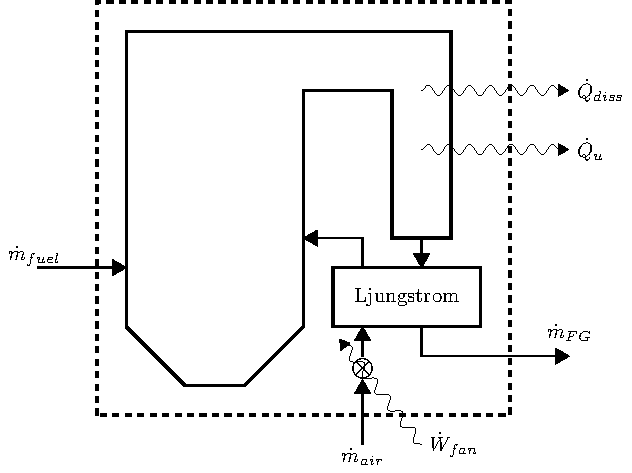
\includegraphics[width=0.8\textwidth]{boiler_fig}
\end{figure}

Writing the total energy balance equation neglecting potential and kinetic energies contribution we get:

\begin{equation}
\dot{H}_{air} + \dot{H}_{fuel} + \dot{m}_{Fuel} \cdot LHV
+ \dot{W}_{fan}
 = \dot{H}_{FG} + \dot{Q}_u + \dot{Q}_{diss}
\end{equation}
To simplify the expression we define 
$\alpha = \dot{m}_{AIR} / \dot{m}_{fuel}$ 
so that we can write 
$\dot{m}_{AIR}$, $\dot{m}_{fuel}$ and 
$\dot{m}_{FG}$ function of $\alpha$ and 
$\dot{m}_{fuel}$.
\begin{center}
\tabulinesep=1.2mm
$\begin{tabu}{|l|l|l|l|}
\hline
\dot{m}        & Air    & Fuel & Flue\ gas \\ \hline
\dot{m}_{fuel} & \alpha & 1    & 1+\alpha  \\ \hline
\end{tabu}$
\end{center}
\begin{equation}
\label{eq:boiler_energy_balance_NG}
\begin{split}
\alpha \cdot \dot{m}_{fuel} \cdot h_{air} \bigg\vert_{T_{ref}}^{T_{air}^{IN}}
 \ +\ 
 \dot{m}_{fuel} \cdot h_{fuel} \bigg\vert_{T_{ref}}^{T_{fuel}^{IN}} 
 \ +\  (1-\eta_{loss}) \cdot \dot{m}_{Fuel} \cdot LHV
 \ +\  \dot{W}_{fan}
 =\\
 (1+\alpha) \cdot \dot{m}_{fuel} \cdot h_{FG} \bigg\vert_{T_{ref}}^{T_{FG}^{ST}}
 \ +\  \dot{Q}_u
\end{split}
\end{equation}

First of all we can get $\alpha$ directly from $\beta_{O_2}$ with the following formula:

\begin{equation}
\alpha
=\frac{\dot{m}_{AIR}}{\dot{m}_{fuel}}
=\beta_{O_2} \cdot \frac{1}{\chi_{O_2}^{air}} \cdot \frac{MM_{air}}{MM_{fuel}} = 18.7157
\end{equation}

We know the enthalpy of each of the species in air, fuel and flue gases,  but we need to know the total enthalpy of the mixtures.

\begin{equation}
 h_{species_i} = \int C_{p_i}dT = \int (A_i+B_i \cdot T)dT 
\end{equation}

\begin{equation}
 h_{mix} = \int C_{p_{mix}}dT = \int (A_{mix}+B_{mix} \cdot T)dT 
\end{equation}
\begin{tabular}{l r}
Where & $\displaystyle A_{mix} = \sum_{i=1}^{species} A_i \cdot y_i$ \\
      & $\displaystyle B_{mix} = \sum_{i=1}^{species} B_i \cdot y_i$ 
\end{tabular}

\begin{center}
\tabulinesep=1.2mm
$\begin{tabu}{|l|l|l|l|}
\hline
  & Air & Fuel & Flue\ gas \\ \hline
A  [\frac{J}{KgK}] & 952.2 & 1052.22 &         1012.39 \\ \hline
B [\frac{J}{Kg}] & 0.1874 & 0.1723 &          0.2756 \\ \hline
\end{tabu}$
\end{center}

Before proceeding to resolve the energy equation we have to choose if to consider $\dot{W}_{fan}$ or to neglect it and then in case we neglect it we will need to verify if this hypothesis is close to reality. We consider \emph{NOT} to neglect $\dot{W}_{fan}$. So we have to evaluate it, knowing that it depends also on $\dot{m}_{fuel}$ that until know is unknown

\begin{equation}
\label{eq:fanpower}
\dot{W}_{fan} = \frac{\Delta p \cdot \dot{m}_{fuel}}{\eta_e \cdot \eta_{fan}} \cdot \left(\frac{\alpha}{\rho^{IN}_{air}} + \frac{1+\alpha}{\rho^{ST}_{FG}}
\right)
\end{equation}
But we have $\Delta p$ in $mm_{H_2O}$ and we have to convert in Pa. Moreover we have to evaluate the density of flue gas and air:\\
[2ex]
\begin{tabular}{l}
 $\displaystyle \Delta p^{(Pa)} = g \cdot 250\,mm_{H_2O} = 2452.5\,Pa$ \\ [2ex]
 $\displaystyle \rho_{air} = \frac{MM_{air} \cdot p}{R \cdot T} 
 = 1.2199 \frac{Kg}{m^3} $ \\[2ex]
 $\displaystyle \rho_{FG} = \frac{MM_{FG} \cdot p}{R \cdot T} 
 = 0.8640 \frac{Kg}{m^3} $
\end{tabular} 
\\

Now the only unknown in $\dot{W}_{fan}$ is the same as energy balance.
Finally we solve equation \ref{eq:boiler_energy_balance_NG} computing $\dot{m}_{fuel}$ and therefore $\dot{m}_{air}$ and $\dot{m}_{FG}$

\begin{center}
\tabulinesep=1.2mm
$\begin{tabu}{|l|l|l|l|}
\hline
  & Air & Fuel & Flue\ gas \\ \hline
\dot{m}  [\frac{Kg}{s}] & 422.75 & 22.59 & 445.34 \\ \hline
\end{tabu}$
\end{center}

We have obtained the value of all our unknown so now we can easy evaluate $\eta_{boiler}$ from equation \ref{eq:etaboiler} :

\begin{equation} 
\eta_{Boiler} = \frac{\dot{Q}_u}{\dot{m}_{fuel} \times LHV} = 95.165\%
\end{equation}

\subsection*{1.d Fan power consumption} 
In equation \ref{eq:fanpower} we have obtained $\dot{m}_{fuel}$ function of $\dot{m}_{fuel}$ that before was unknown. Now instead we can correctly evaluate the power of fan:

\begin{equation}
\dot{W}_{fan} = \frac{\Delta p \cdot \dot{m}_{fuel}}{\eta_e \cdot \eta_{fan}} \cdot (\frac{\alpha}{\rho^{IN}_{air}} + \frac{1+\alpha}{\rho^{ST}_{FG}}
) = 2.94 MW
\end{equation}

\subsection*{1.e $T_{air}$ at Ljungstrom outlet} 
\begin{figure}[h]
  \caption{Ljungstrom flow Scheme.}
  \centering
  \usetikzlibrary{decorations.pathmorphing}
\usetikzlibrary{decorations.markings}
\usetikzlibrary{decorations.pathmorphing}
\usetikzlibrary{arrows}
\begin{tikzpicture}[>=triangle 60]
% rectangle
\draw[very thick] (0,0) rectangle (5,3);
% air line
\draw[->]  (-1,2)--(1,2);
\draw[decorate,decoration=zigzag] (1,2)--(4,2);
\draw[->]  (4,2)--(6,2);
% flue gas linetriangle 60
\draw[<-]  (-1,1)--(1,1);
\draw[decorate,decoration=zigzag] (1,1)--(4,1);
\draw[<-]  (4,1)--(6,1);
%
\node[left] at (-1.5,2) {Air};
\node[left] at (-1.5,1) {Flue gas};
% heat transfer
\draw[red, decorate,decoration=snake] (2.5,2.5)--(2.5,0.5);
\draw[red,->]  (2.5,2.5)--(2.5,2.7);
\node[red,left] at (2.4,2.6) {$\dot{Q}$};
\end{tikzpicture}
\end{figure}

We know $T_{air}^{IN}$, $T_{FG}^{IN}$, $T_{FG}^{OUT}$ and we miss only $T_{air}^{OUT}$. We can get $T_{air}^{OUT}$ with an energy balance over the Ljungstrom:

\begin{equation}
\label{eq:ljungstrom_balance}
\dot{H}_{air} 
= \dot{m}_{air} \cdot \int_{T_{air}^{IN}}^{T_{air}^{OUT}} C_{p_{air}}dT 
= \dot{m}_{FG} \cdot \int_{T_{FG}^{IN}}^{T_{FG}^{OUT}} C_{p_{FG}}dT 
= \dot{H}_{FG}
\end{equation}
Where IN and OUT refer to the inlet and the outlet of the Ljungstrom.

To solve the equation respect of our unknown we can or evaluate the integral and than solve the second order algebraic equation, or in term of generality we can simply us a numeric method like Secant one. We Matlab support we have considered to proceed with the second opportunity. Therefore we have obtained the following result:

\begin{equation}
T_{air}^{OUT} = 237.96 ^{\circ}C
\end{equation}
So finally we can draw the temperature-heat plot 
\begin{figure}[h]
  \centering
  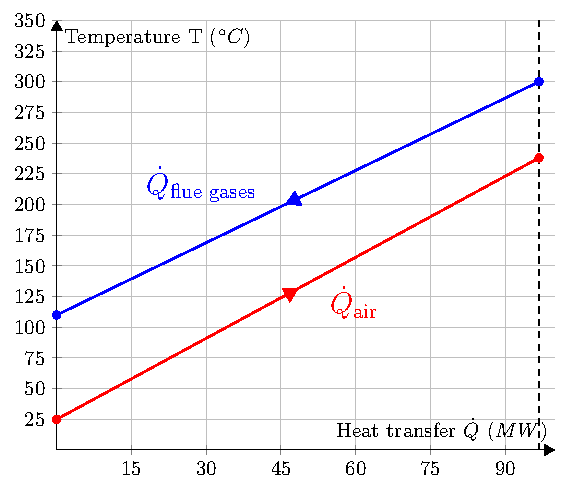
\includegraphics{ljungstrom_plot_fig.pdf}
  \caption[scale=0.5]{Ljungstrom temperature-heat exchanger plot.}
\end{figure}

In this analysis we have neglected the fact that the fan increase a bit the temperature of air.

\subsection*{1.f Flame adiabatic temperature} 
To compute the flame adiabatic temperature we need to make an energy balance around the flame:
Because the request is about \emph{adiabatic} temperature we do not consider losses.

\begin{figure}[h]
 \centering
  \caption{Flame flow scheme.}
  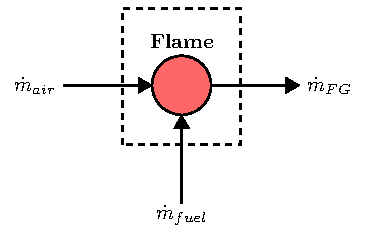
\includegraphics[scale=1]{flame_temp_fig.pdf}
\end{figure}
\vspace*{-0.5cm}
\begin{equation}
\dot{H}_{air} + \dot{H}_{fuel} + \dot{m}_{fuel} \cdot LHV = \dot{H}_{FG}
\end{equation}
\begin{equation}
\dot{m}_{air} \cdot h_{air}\bigg\vert_{T_{ref}}^{T_{air}^{PH}} +
\dot{m}_{fuel} \cdot \left(LHV + h_{fuel}\bigg\vert_{T_{ref}}^{T_{fuel}^{IN}}\right)
 = \dot{m}_{FG} \cdot h_{fuel}\bigg\vert_{T_{ref}}^{\boldsymbol{T_{flame}} } 
\end{equation}

We can solve this equation numerically like equation \ref{eq:ljungstrom_balance}. So we can get $T_{flame}$ with secants method:

\begin{equation}
T_{flame} = 1924.54 ^{\circ}C
\end{equation}

\subsection*{Solution for Coal firing}

\subsection*{2.a Flue gas composition at the outlet of the boiler} 
In this case we have a solid fuel; we do not have the molecular composition of our fuel but from a \emph{chemical analysis} we got the mass fraction of each atoms in coal. First of all it is necessary to evaluate for each atom the molar fraction respect to carbon. We take carbon as reference because we are sure to have it in every fossil fuel.

\begin{equation}
n_i = \left[\frac{Kmols_i}{Kmols_C}\right] = \frac{y_i}{y_C}
 \cdot \frac{MM_c}{MM_i}
\end{equation}

Where $y_i$ is the mass fraction of $i$.\\ Moreover the molar fraction respect of fuel of each atom ($\chi_i$) is computed as:

\begin{equation}
\chi_i = y_i
 \cdot \frac{MM_{fuel}}{MM_i}
\end{equation}
Where $ {MM_{fuel}} = \sum_{i=1}^{n_{species\ in\ fuel}}\chi_i \cdot MM_i = 12.22 \frac{Kg}{Kmol}$  \\

The results are reported in the following table.
\begin{center}
\begin{tabu}{|c|c|c|c|c|c|c|}
\hline
     & $ C $ & $ H $ & $ O $ & $ N $ & $ S $ & $Moisture$\\ \hline
 $n$ & 1 & 0.912 & 0.108 & 0.0154 & 0.0208 & 0.131 
\\ \hline
 $\chi$ & 62.38$\%$ & 56.90$\%$ & 6.75$\%$ & 0.96$\%$ & 1.30$\%$ & 8.145$\%$
 \\ \hline
\end{tabu}
\end{center}
Before writing the complete equation of reaction we need to evaluate $\beta_{O_2}$, the required moles of $O_2$ to have a stoichiometric oxidation reaction:

\begin{equation}
\beta_{O_2} = (1+\varepsilon) \cdot \beta_{O_2}^{Stoichiometric} 
=(1+\varepsilon) \cdot \left( N_C + \frac{N_H}{4} + N_S - N_{O_2} \right)= ...
\end{equation}

Now we can write the complete equation of reaction; we have neglected $SO_3$ which has low molar fraction and it is significant only as regarding acids formation that corrode tubes:
\begin{equation}
\begin{split}
CH_{n_H}O_{n_O}N_{n_N}S_{n_S} +\chi^{fuel}_{H_2O}H_2O + \beta_{O_2} \cdot
(O_2 + \frac{\chi_{N_2}}{\chi_{O_2}}N_2 + 
\frac{\chi_{Ar}}{\chi_{O_2}}Ar + \frac{\chi^{air}_{H_2O}}{\chi_{O_2}}H_2O
) = 
\\
aCO_2 + bH_2O + cN_2 + dAr + eSO_2 + fO_2
\end{split}
\end{equation}

Where $a,b,c,d$ and $e$ are the unknowns. Balancing the reaction we can get them:
 
\begin{center}
$\begin{tabu}{|l|c|c|c|c|c|c|}
\hline
 & a\ (CO_2)  &  b\ (H_2O)  &  c\ (N_2)  &  d\ (Ar) & e\ (SO_2) & f\ (O_2) \\ \hline
n & 1 & 0.667 & 5.771 & 0.0723 & 0.0209 & 0.347
 \\ \hline
\end{tabu}$
\end{center}

Finally we can get $\chi$ and $y$ of each species in the flue gases remembering that $\chi_i = \frac{n_i}{\sum n_i}$ and $y_i = \chi_i\times \frac{MM_i}{MM_{FG}}$

\begin{center}
%\begin{tabu}{|l|{c|}*{6}}
\begin{tabu}{|l|c|c|c|c|c|c|}
\hline
     & $ CO_2 $ & $ H_2O $ & $ N_2 $ & $ Ar $ & $ SO_2 $ & $ O_2 $\\ \hline
 $\chi$ & $12.69\%$ & $8.46\%$ & $73.26\%$ & $0.918\%$ & $0.265\%$ & $4.40\%$\\ \hline
\end{tabu}
\end{center}

\subsection*{2.b Efficiency of boiler considering} 
The efficiency is defined as the useful output over the total input, or in formulas it is:

\begin{equation} 
\label{eq:etaboiler_coal}
\eta_{Boiler} = \frac{\dot{Q}_u}{\dot{m}_{Fuel} \times LHV}
\end{equation}
But if $\dot{Q}_u$ is a data of the problem $\dot{m}_{Fuel}$ is unknown. To evaluate it is necessary to compute an energy balance over the total boiler.

\begin{figure}[h]
  \caption{Energy and mass flows through the boiler.}
  \centering
    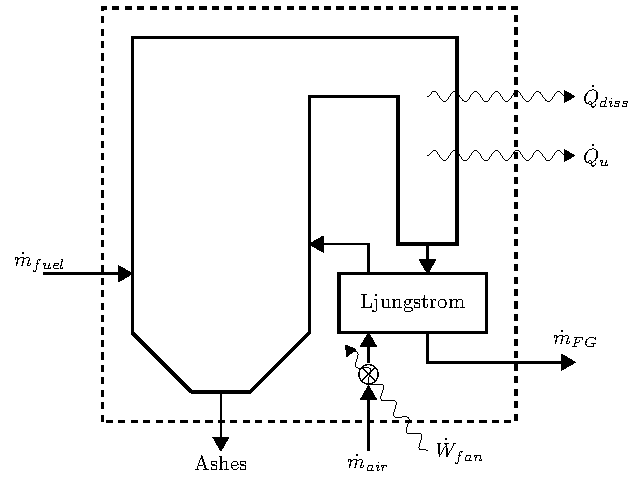
\includegraphics[width=0.8\textwidth]{boiler_coal_fig}
\end{figure}

Writing the total energy balance equation we get:

\begin{equation}
\dot{H}_{air} + \dot{H}_{fuel} + \dot{m}_{Fuel} \cdot LHV 
 + \dot{W}_{fan}
 = \dot{H}_{FG} + \dot{H}_{ash} + \dot{Q}_u + \dot{Q}_{diss}
\end{equation}
The ashes do not react with other species in the chemical reaction, but instead they are significant from the energy point of view because ashes absorb energy generated in the combustion process.
\begin{equation}
\label{eq:coal_energy_balance_boiler}
\begin{split}
\alpha \cdot \dot{m}_{Fuel} \cdot h_{air} \bigg\vert_{T_{ref}}^{T_{air}^{IN}}
 \ +\ 
 \dot{m}_{fuel} \cdot \cancel{ h_{fuel}\bigg\vert_{T_{ref}}^{T_{fuel}^{IN}} }
 \ +\  (1-\eta_{loss}) \cdot \dot{m}_{Fuel} \cdot LHV
 \ +\  \dot{W}_{fan}
 =\\
 (1+\alpha) \cdot \dot{m}_{fuel} \cdot h_{FG} \bigg\vert_{T_{ref}}^{T_{FG}^{ST}} \ +\ 
 y_{ash} \cdot \dot{m}_{fuel} \cdot Cp_{ash} (T_{ash}^{OUT} - T_{ref} )
 \ +\  \dot{Q}_u
\end{split}
\end{equation}
$h_{fuel}$ contribute is negligible respect of LHV.
In this case we miss both the $\dot{m_i}$ and the  

First of all we can get $\alpha$ directly from $\beta_{O_2}$ with the following formula:

\begin{equation}
\alpha = \beta_{O_2} \cdot \frac{1}{\chi_{O_2}^{air}} \cdot \frac{MM_{air}}{MM_{C}} \cdot y_C = 10.96
\end{equation}

We know the enthalpy of each of the species in air, fuel and flue gases,  but we need to know the total enthalpy of the mixtures.

\begin{equation}
 h_{species_i} = \int C_{p_i}dT = \int (A_i+B_i \cdot T)dT 
\end{equation}

\begin{equation}
 h_{mix} = \int C_{p_{mix}}dT = \int (A_{mix}+B_{mix} \cdot T)dT 
\end{equation}
\begin{tabular}{l r}
Where & $\displaystyle A_{mix} = \sum_{i=1}^{species} A_i \cdot y_i$ \\
      & $\displaystyle B_{mix} = \sum_{i=1}^{species} B_i \cdot y_i$ 
\end{tabular}

\begin{center}
\tabulinesep=1.2mm
$\begin{tabu}{|l|c|c|c|}
\hline
  & Air & Ash & Flue\ gas \\ \hline
A  [\frac{J}{KgK}] & 952.2 & 2000 & 947.23 \\ \hline
B [\frac{J}{Kg}] & 0.1874 & 0 & 0.2790 \\ \hline
\end{tabu}$
\end{center}

Unlike the previous case with natural gas we do not know the temperature at which the flue gas goes out from our control volume. We can obtain it considering that it must be at least $25^{\circ}C$ more than dew point temperature of $SO_2$ and $SO_3$. So we proceed to evaluate that temperature.

\begin{equation*}
T_{H_2SO_4} = \frac{1000}{2.276-0.0294 \cdot \log(p_{H_2O})
+0.0858 \cdot \log(p_{SO_3})
-0.00062 \cdot \log(p_{H_2O})\log(p_{SO_3})}
\end{equation*}

\begin{equation*}
T_{H_2SO_3}=\frac{1000}{3.9526-0.1863 \cdot \log(p_{H_2O})+0.000867 \cdot \log(p_{SO_2})-0.000913 \cdot \log(p_{H_2O})\log(p_{SO_2})}
\end{equation*}
But we do not know $p_{SO_2}$ and $p_{SO_2}$. We can calculate them with the assumption that they are ideal gases. So the partial pressure is just the total pressure multiplied by the molar fraction.
\begin{align} 
p_{SO_2} &= \left( 1-\frac{2.5}{100} \right) \cdot \chi_{SO_2} \cdot p_{ATM} =1.980\,bar\\ 
p_{SO_3} &= \frac{2.5}{100} \cdot \chi_{SO_2} \cdot p_{ATM} = 0.0508\,bar
\end{align}
\begin{flalign*}
\text{Finally we obtain that } T_{H_2SO_3} &=315.06\,K &\\ 
							   T_{H_2SO_4} &=416.41\,K &
\end{flalign*}.
We must impose an outlet temperature at the stack $25 \celsius$ greater than the maximum dew point temperature so:

\begin{equation}
T_{FG}^{ST} = \left(25\,K + T_{H_2SO_4} \right)=441.41\,K=168.26\celsius 
\end{equation}

Before proceeding to resolve the energy equation \ref{eq:coal_energy_balance_boiler} we have to choose if to consider $\dot{W}_{fan}$ or to neglect it and then verify if this hypothesis is close to reality. We consider \emph{NOT} to neglect $\dot{W}_{fan}$. So we have to evaluate it, knowing that it depends also on $\dot{m}_{fuel}$. We proceed in the same way as equation \ref{eq:fanpower} considering that $\Delta p$ now is $350\ mm_{H_2O}$.

\begin{equation}
\label{eq:fanpower_coal}
\dot{W}_{fan} = \frac{\Delta p \cdot \dot{m}_{fuel}}{\eta_e \cdot \eta_{fan}} \cdot \left(\frac{\alpha}{\rho^{IN}_{air}} + \frac{1+\alpha}{\rho^{ST}_{FG}}
\right)
\end{equation}

Now we can solve equation \ref{eq:coal_energy_balance_boiler} where the only unknown is $\dot{m}_{fuel}$, because also $\dot{W}_{fan}$ depends only on $\dot{W}_{fan}$. Finally we can compute $\dot{m}_{fuel}$ and therefore $\dot{m}_{air}$ and $\dot{m}_{FG}$.

\begin{table}[h]
\centering
\tabulinesep=1.2mm
$\begin{tabu}{|l|c|c|c|}
\hline
  & Air & Fuel & Flue\ gas \\ \hline
\dot{m}  \left[\frac{kg}{s}\right] & 481.49 & 43.85 & 525.35 \\ \hline
\end{tabu}$
\caption{Mass flow rates}
\label{table:m_dot_coal}
\end{table}

We have obtained the value of all our unknown so now we can easy evaluate $\eta_{boiler}$ from equation \ref{eq:etaboiler} :

\begin{equation} 
\eta_{Boiler} = \frac{\dot{Q}_u}{\dot{m}_{fuel} \times LHV} = 91.86\%
\end{equation}

\subsection*{2.c Fan power consumption} 
In equation \ref{eq:fanpower_coal} we have obtained $\dot{W}_{fan}$ function of $\dot{m}_{fuel}$,that before was unknown, and $\dot{m}_{fuel}$ from table \ref{table:m_dot_coal}. Now instead we can correctly evaluate the power of fan:

\begin{equation}
\dot{W}_{fan} = \frac{\Delta p \cdot \dot{m}_{fuel}}{\eta_e \cdot \eta_{fan}} \cdot \left(\frac{\alpha}{\rho^{IN}_{air}} + \frac{1+\alpha}{\rho^{ST}_{FG}}
\right) = 5.06 MW
\end{equation}

\end{document}
